\bigskip 
\bigskip 
\subsubsection{Contenido}
\bigskip 
%\begin{wrapfigure}{r}{0.5\textwidth}
%  \begin{center}
%    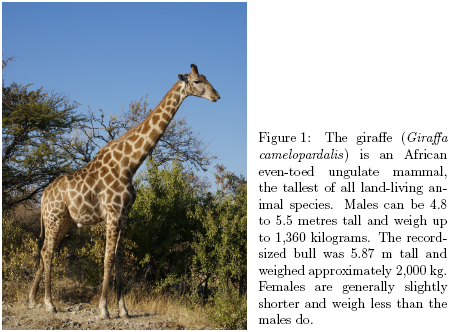
\includegraphics[width=0.48\textwidth]{./ingles/Latex_example_sidecap.jpg}
%  \end{center}
%\end{wrapfigure}

\begin{description}
\item[Nombre:] Volga
\item[Cristaleria:] Vaso Largo (10oz / 300cc)
\item[M\'etodo de elaboraci\'on:] Directo
\item[Decoraci\'on:] Sin decoraci\'on.
\end{description}

\begin{table}[h]
\caption{Ingredientes y proporciones} 
\label{tab:fonts}
\begin{center}       
\begin{tabular}{|l|l|l|c|l|} %% this creates two columns
%% |l|l| to left justify each column entry
%% |c|c| to center each column entry
%% use of \rule[]{}{} below opens up each row
\hline
\rule[-1ex]{0pt}{3.5ex}  \textbf{Producto} & \textbf{Bebida} & \textbf{Marca} & \textbf{Volumen} & \textbf{Fraccion}  \\
\hline
\rule[-1ex]{0pt}{3.5ex}  Aguardiente & Vodka 			& Wyborowa 		& 2 1/2 oz / 85 cc 	&  	\\
\hline
\rule[-1ex]{0pt}{3.5ex}  Licor 		& Menta	 	& Bols		& 1 oz / 30 cc 		&  	\\
\hline
\rule[-1ex]{0pt}{3.5ex}  Gaseosa	& Agua T\'onica 	& Schweppes 				& 5 oz / 150 cc		& 	\\
\hline

\end{tabular}
\end{center}
\end{table} 
\bigskip 

%%-----------------------------------------------------------
\subsubsection{Formato de elaboraci\'on} 
\label{sec:title}
\bigskip 
\begin{center}
\begin{enumerate}
\item Colocar el vodka y luego el licor en un vaso de trago largo.
\item Colocar las 5 oz de t\'onica, y rellenar con hielo picado.
\end{enumerate}
\end{center}
\bigskip 
\bigskip 
%%%%%%%%%%%%%%%%%%%%%%%%%%%%%%%%%%%%%%%%%%%%%%%%%%%%%%%%%%%%%

\subsubsection{Notas}
\bigskip 
\begin{center}
\raggedright{}Servir con sorbete.
\end{center} 